\documentclass[tikz]{standalone}% 'crop' is the default for v1.0, before it was 'preview'
\usepackage{tikz}
\usepackage{pgfplots}
\usepackage{amsmath}

\usepgfplotslibrary{colormaps}
\pgfplotsset{compat=1.18}
\usetikzlibrary{plotmarks, arrows.meta, shapes}
%\usetikzlibrary{...}% tikz package already loaded by 'tikz' option
\begin{document}


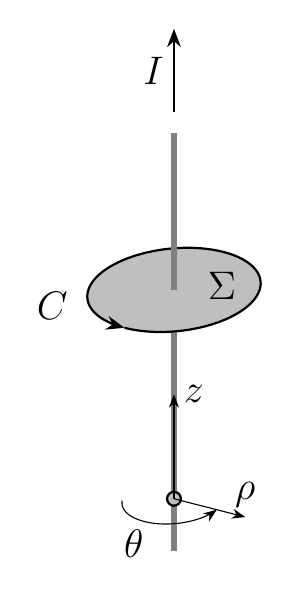
\begin{tikzpicture}[font=\Large]
  \begin{axis}[
    view={120}{40},
    hide axis,
    scale=2,
    xmin=-2, xmax=2, ymin=-2, ymax=2, zmin=0, zmax=4,
    enlarge y limits=0.1,
  ]

    % Line charge (vertical line)
    \addplot3[line width=2pt, color=black!50]
      coordinates {(0,0,0) (0,0,4)};  % vertical line through origin
    \draw[thick, ->, >=Stealth] (axis cs:0,0,4.2) -- (axis cs:0,0,5) node[midway, left] {$I$};

    \addplot3[black, thick, ->, >=Stealth, fill=black!25, variable=\t, domain=0:360, samples=100, samples y=1] ( {0.5*cos(t)}, {0.5*sin(t)}, {2.5});
    \node[left] at (axis cs: 0.4,-0.4,2.5) {$C$};
    \addplot3[line width=2pt, color=black!50]
      coordinates {(0,0,2.5) (0,0,4)};  % vertical line through origin
    \node[right] at (axis cs: -0.1,0.1,2.5) {$\Sigma$};


    \node[circle,draw=black, thick, fill=black!25,inner sep=0pt,minimum size=5pt] at (axis cs: 0,0,0.5) {}; 

    \addplot3[black, ->, >=Stealth, variable=\t, domain=-60:90, samples=50, samples y=1] ( {0.3*cos(t)}, {0.3*sin(t)}, {0.5});
    \node[left] at (axis cs: 0.5,0.2,0.5) {$\theta$};
    \draw[->, >=Stealth] (axis cs:0,0,0.5) -- (axis cs:0,0.5,0.5) node[above] {$\rho$};
    \draw[->, >=Stealth] (axis cs:0,0,0.5) -- (axis cs:0,0,1.5) node[right] {$z$};
  \end{axis}


\end{tikzpicture}
\end{document}